\chapter{Szimulációk, eredmények}

A szimulációs és szomszédossági mátrixos ábrákon a matplotlibes plazma
színezésnek megfelelően a hidegebb (kék) árnyalatok kisebb értéket, a melegebb
(lila, majd sárga) árnyalatok magasabb értékeket jelölnek. A fehér szín a 0
értéket jelöli. A gráfok és részgráfok ábrái $n \times n$-es szomszédossági
mátrixokat ábrázolnak. A fehér cellák a nem-élek, a kék cellák az $1$-es súlyú
élek. A szimulációk ábráinak az $x$ tengelyén a gráfok csúcsai helyezkednek el
kiterítve, index szerinti növekvő sorrendben, az $y$ tengelyen a szimuláció
lépései helyezkednek el, alul a $0.$ lépés, felül az utolsó lépés.

\section{Súlyzó gráf}

A félév során először a súlyzón implementáltam a klasszikus bolyongást. Ez a
gráf két körből áll, a két kör csúcsainak egy-egy részhalmazát egy teljes páros
gráf kapcsolja össze. Az alábbiakban a nevesített részgráfok, illetve a teljes
gráf szomszédossági mátrixai láthatók.

\begin{figure}[H]
  \centering
  \begin{subfigure}{.3\linewidth}
    \centering
    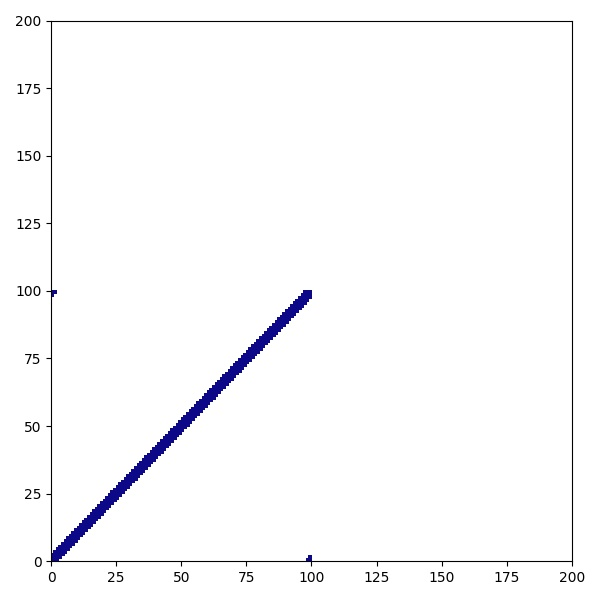
\includegraphics[width=\linewidth]{./figures/sulyzo/subgraph_00.jpg}
    \caption{Bal kör}
    \label{fig:sub1}
  \end{subfigure}
  \begin{subfigure}{.3\linewidth}
    \centering
    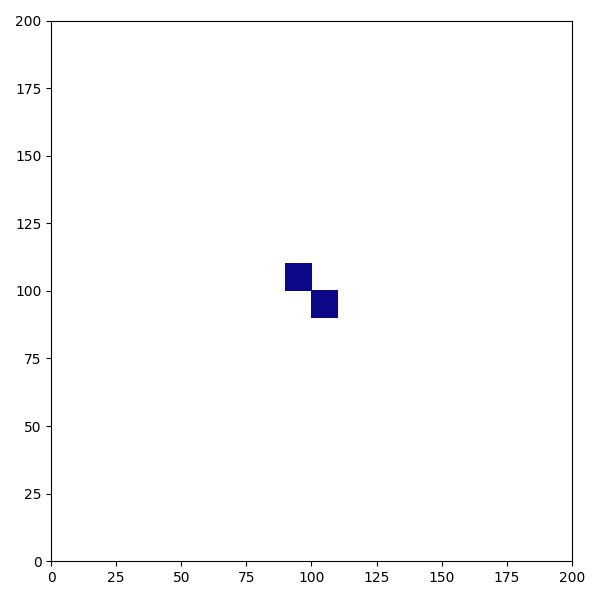
\includegraphics[width=\linewidth]{./figures/sulyzo/subgraph_02.jpg}
    \caption{Középső teljes páros gráf}
    \label{fig:sub2}
  \end{subfigure}
  \begin{subfigure}{.3\linewidth}
    \centering
    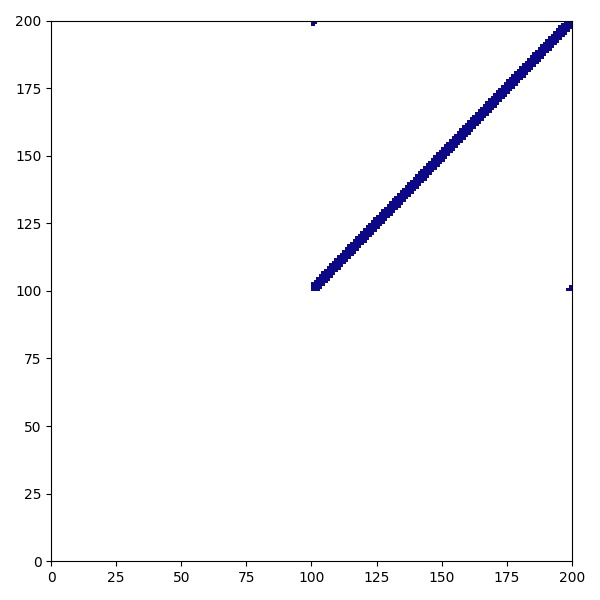
\includegraphics[width=\linewidth]{./figures/sulyzo/subgraph_01.jpg}
    \caption{Jobb kör}
    \label{fig:sub3}
  \end{subfigure}
  \caption{Súlyzó gráf részgráfjai}
  \label{fig:all}
\end{figure}

\begin{figure}[H]
  \centering
  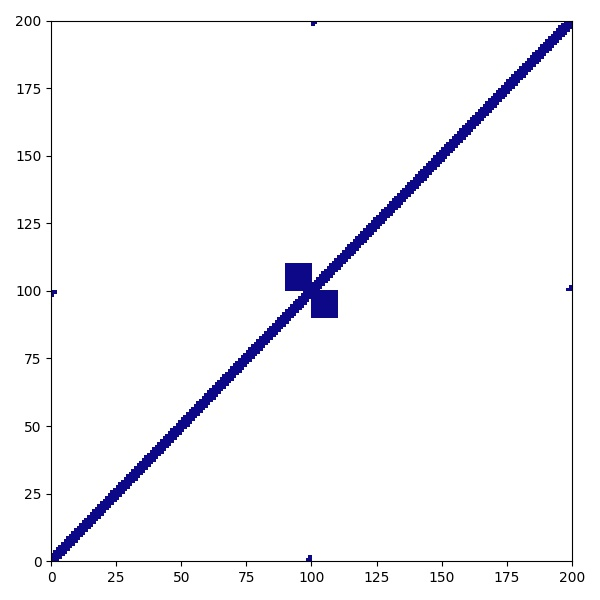
\includegraphics[width=0.5\linewidth]{./figures/sulyzo/graph.jpg}
  \caption{Súlyzó gráf}
\end{figure}

A szimulációkat 1, 10, 100, illetve 1000 darab bolyongóval is elvégeztem,
mindig az $x$ tengelyen középső csúcsból indítva a futtatásokat. Az 1 bolyongós
képen látszik, hogy a szimuláció során sokáig időzik a középső teljes páros
gráf élein lépkedve. Ennek az az oka, hogy az ottani csúcsok fokszámának
jelentős részét a páros gráf élei adják ki, a kör élei sokkal kevesebben
vannak.

\begin{figure}[H]
  \centering
  \begin{subfigure}{.4\linewidth}
    \centering
    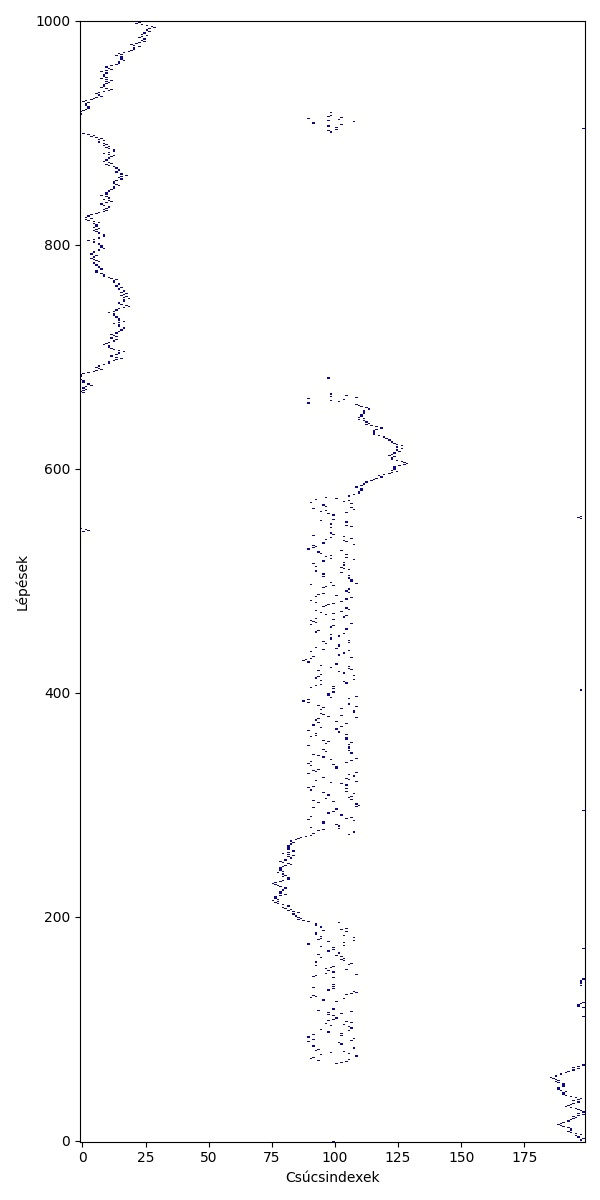
\includegraphics[width=\linewidth]{./figures/sulyzo/sim00.jpg}
    \caption{1 bolyongó}
  \end{subfigure}
  \begin{subfigure}{.4\linewidth}
    \centering
    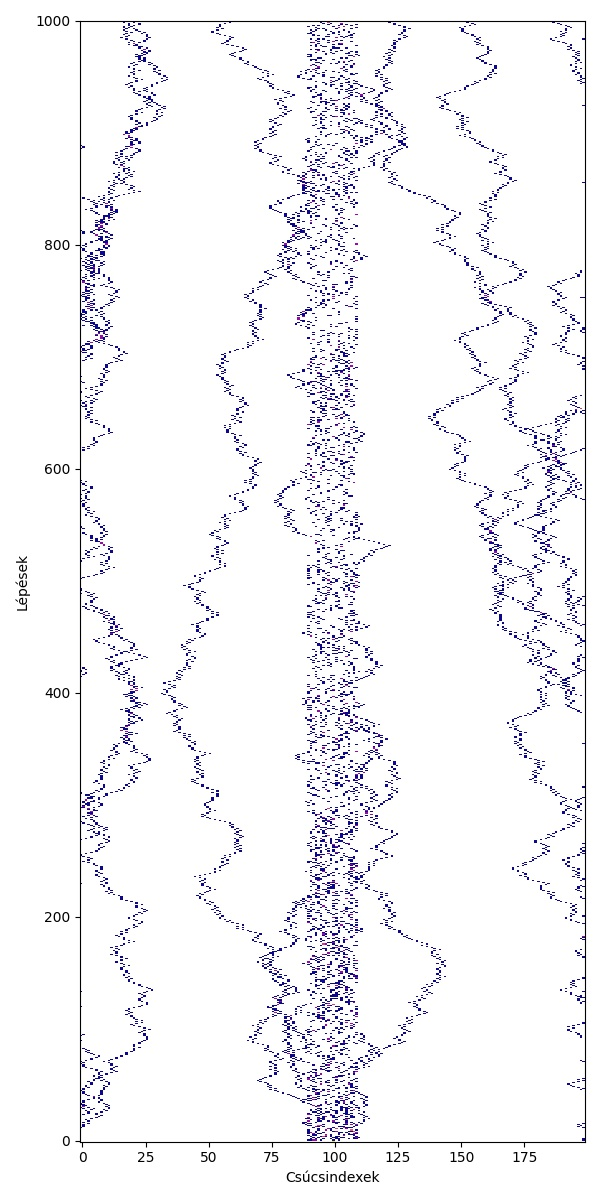
\includegraphics[width=\linewidth]{./figures/sulyzo/sim01.jpg}
    \caption{10 bolyongó}
  \end{subfigure}
\end{figure}

Az 1000 bolyongós képen az eloszlás alakulása figyelhető meg. Látható, hogy a
középső sáv sokkal ,,forróbb'', az ide bekerülő bolyongók sokáig nem jutnak ki.

\begin{figure}[H]
  \centering
  \begin{subfigure}{.4\linewidth}
    \centering
    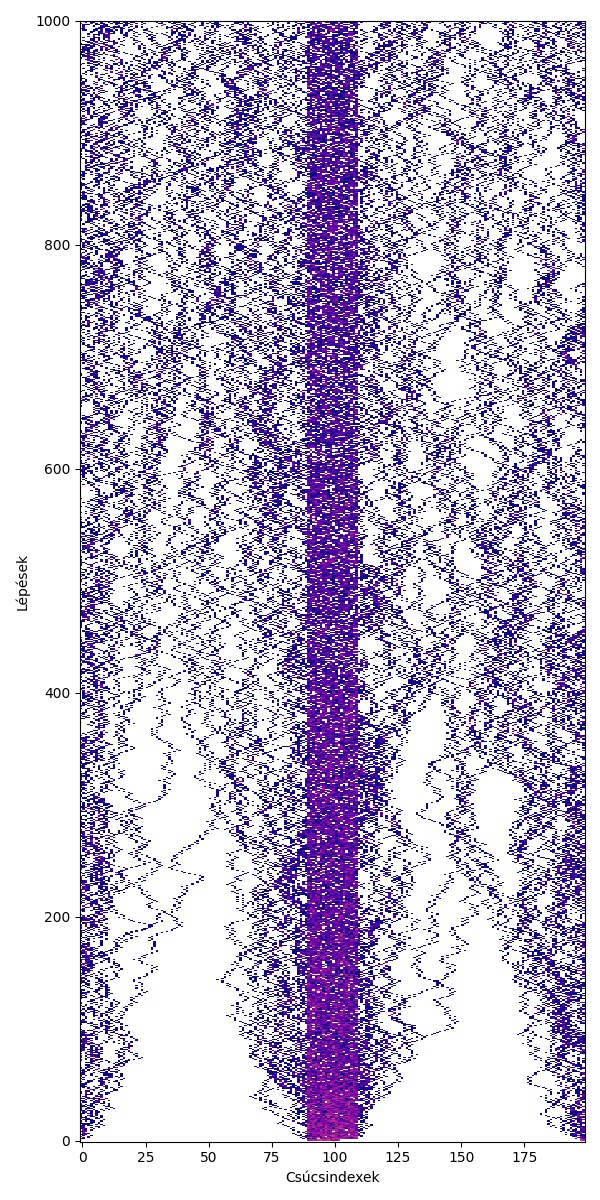
\includegraphics[width=\linewidth]{./figures/sulyzo/sim02.jpg}
    \caption{100 bolyongó}
  \end{subfigure}
  \begin{subfigure}{.4\linewidth}
    \centering
    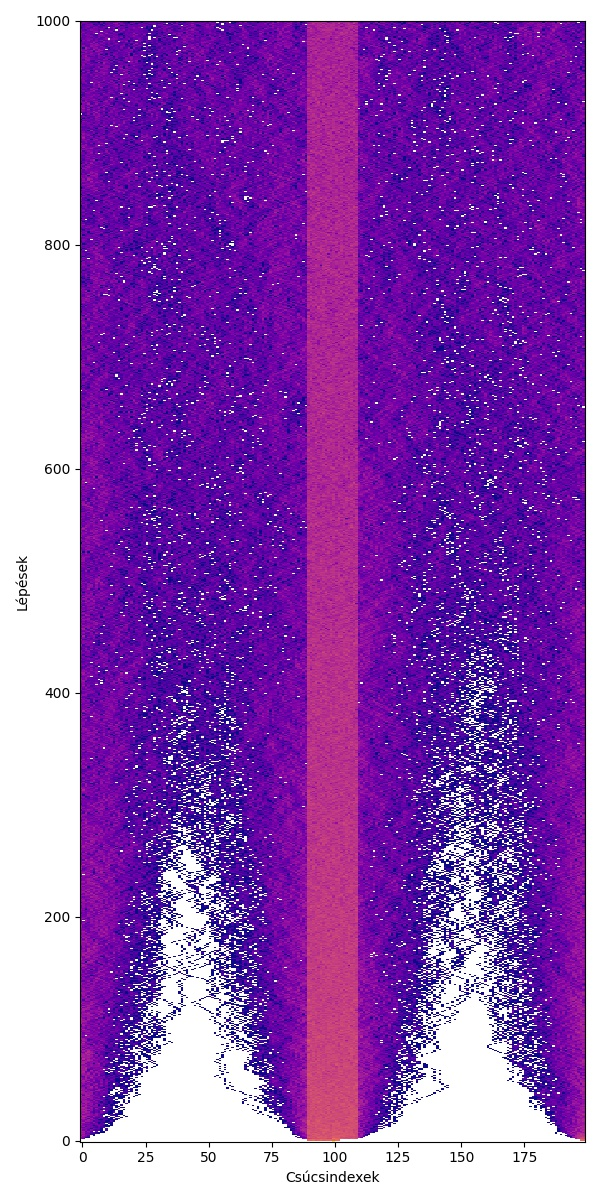
\includegraphics[width=\linewidth]{./figures/sulyzo/sim03.jpg}
    \caption{1000 bolyongó}
  \end{subfigure}
\end{figure}

\section{Ragasztott bináris fa}

A félév során implementáltam még a ragasztott bináris fán történő klasszikus
bolyongást is. Az alábbi ábrákon látható a két teljes bináris fa, a leveleik között
lévő teljes páros gráf, illetve az egész gráf szomszédossági mátrixsza.

\begin{figure}[H]
  \centering
  \begin{subfigure}{.3\linewidth}
    \centering
    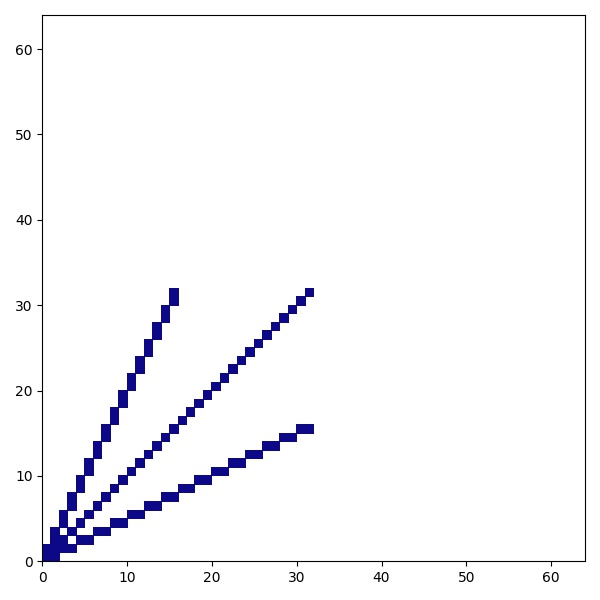
\includegraphics[width=\linewidth]{./figures/ragasztott_binaris/subgraph_00.jpg}
    \caption{Bal bináris fa}
  \end{subfigure}
  \begin{subfigure}{.3\linewidth}
    \centering
    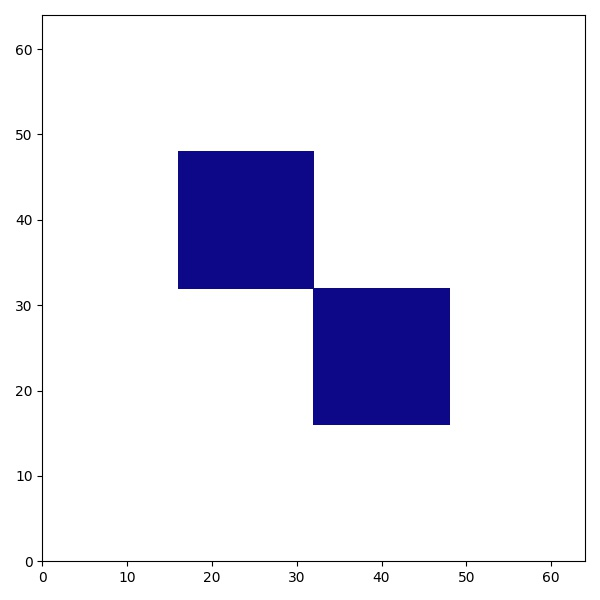
\includegraphics[width=\linewidth]{./figures/ragasztott_binaris/subgraph_02.jpg}
    \caption{Középső teljes páros gráf}
  \end{subfigure}
  \begin{subfigure}{.3\linewidth}
    \centering
    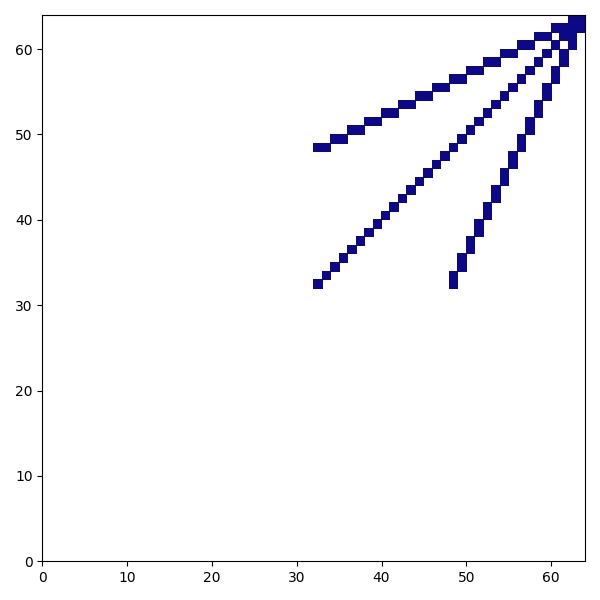
\includegraphics[width=\linewidth]{./figures/ragasztott_binaris/subgraph_01.jpg}
    \caption{Jobb bináris fa}
  \end{subfigure}
  \caption{Ragasztott bináris fa részgráfjai}
\end{figure}

\begin{figure}[H]
  \centering
  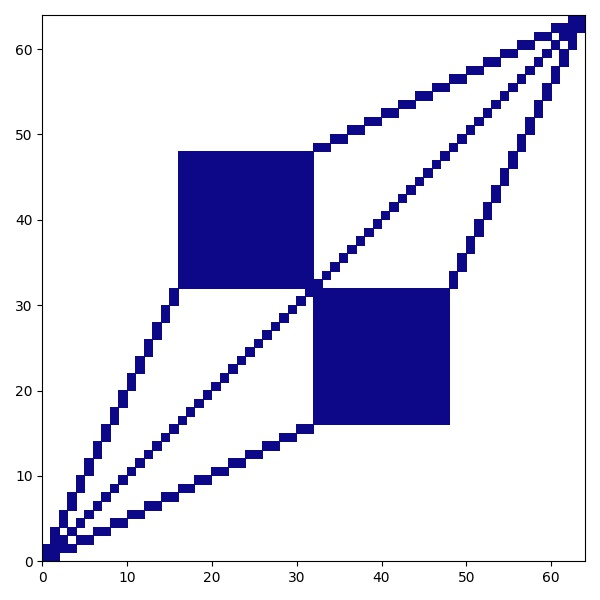
\includegraphics[width=0.5\linewidth]{./figures/ragasztott_binaris/graph.jpg}
  \caption{Ragasztott bináris fa}
\end{figure}

A szimulációt itt most a $0.$ csúcsból indítottam, hasonlóan az előzőekhez
1, 10, 100 és 1000 bolyongóra.

\begin{figure}[H]
  \centering
  \begin{subfigure}{.40\linewidth}
    \centering
    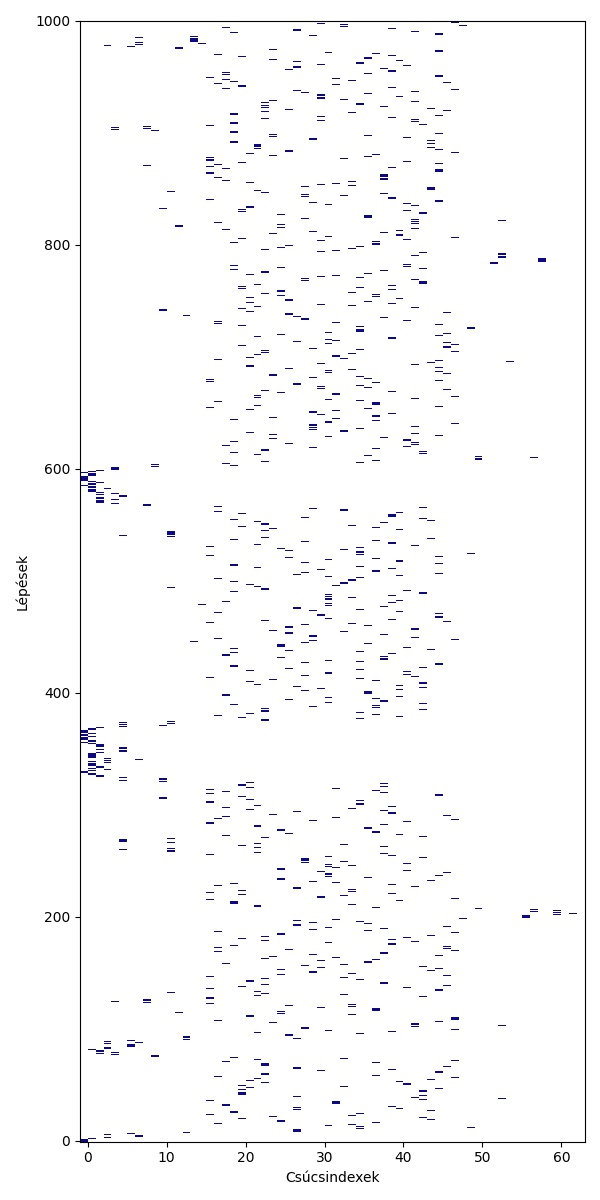
\includegraphics[width=\linewidth]{./figures/ragasztott_binaris/sim00.jpg}
    \caption{1 bolyongó}
  \end{subfigure}
  \begin{subfigure}{.40\linewidth}
    \centering
    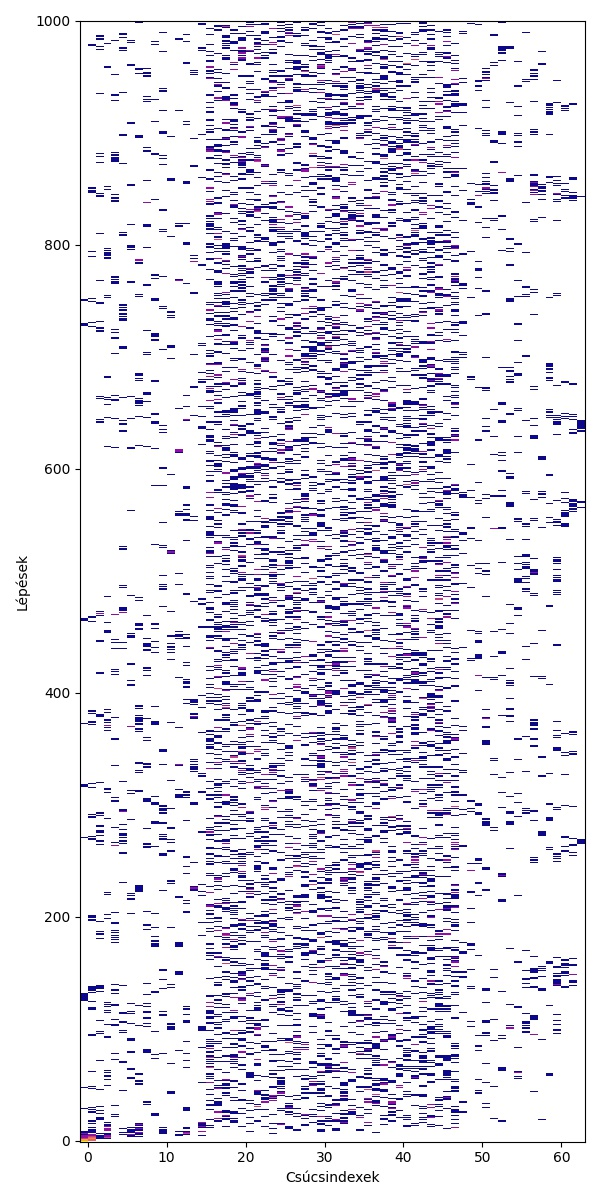
\includegraphics[width=\linewidth]{./figures/ragasztott_binaris/sim01.jpg}
    \caption{10 bolyongó}
  \end{subfigure}
\end{figure}

\begin{figure}[H]
  \centering
  \begin{subfigure}{.40\linewidth}
    \centering
    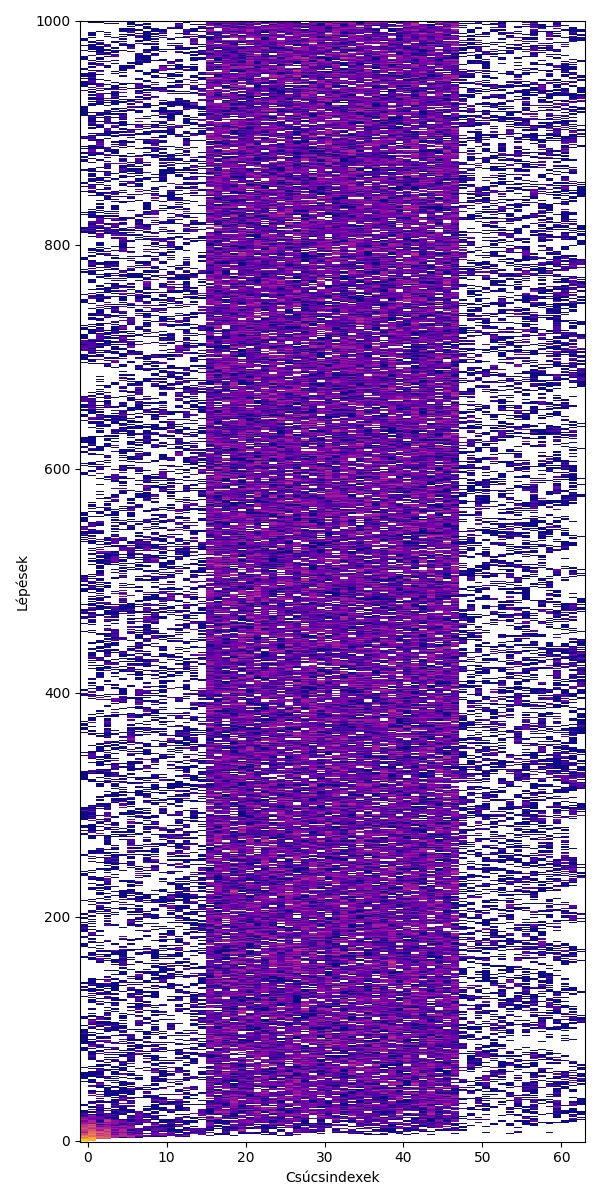
\includegraphics[width=\linewidth]{./figures/ragasztott_binaris/sim02.jpg}
    \caption{100 bolyongó}
  \end{subfigure}
  \begin{subfigure}{.40\linewidth}
    \centering
    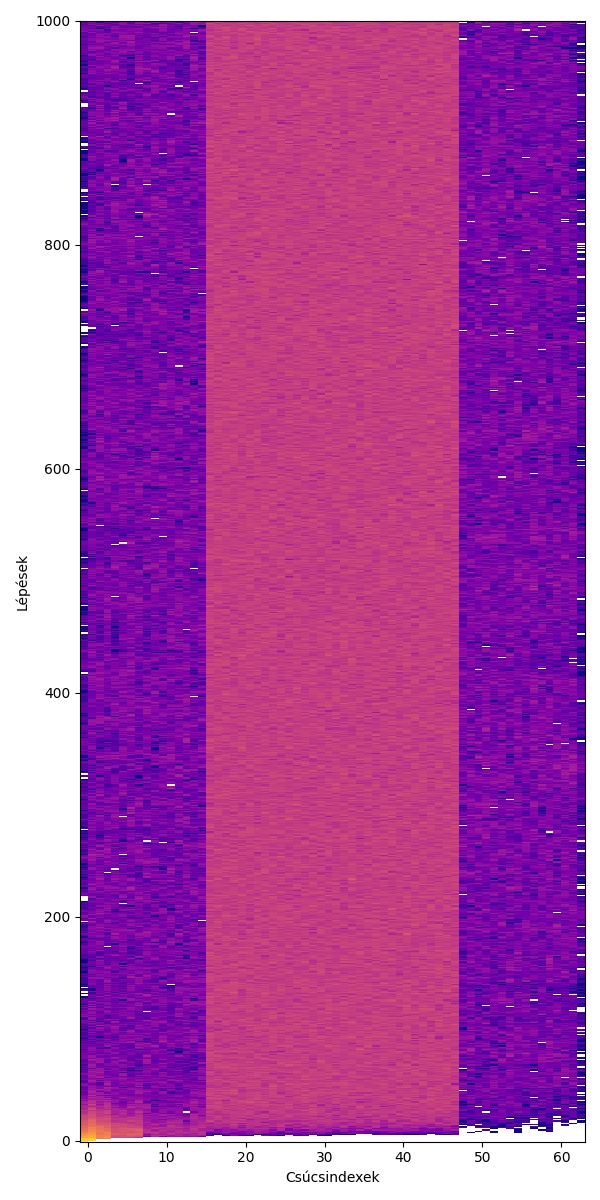
\includegraphics[width=\linewidth]{./figures/ragasztott_binaris/sim03.jpg}
    \caption{1000 bolyongó}
  \end{subfigure}
\end{figure}

\section{Bolyongás az egyenesen, klasszikus és kvantum esetben}

A 4. fejezetben ismertetett egyenesen történő kvantumbolyongás algoritmusát
implementáltam klasszikus, illetve kvantumos esetben is. Az alábbi szimulációs
ábrákon látható, hogy klasszikus esetben az eloszlás úgy alakul, hogy az origó
környékén ,,púposodik'', míg kvantum esetben két ,,púpja'' van, az origótól
messze, arra szimmetrikusan.

\begin{figure}[H]
  \centering
  \begin{subfigure}{.45\linewidth}
    \centering
    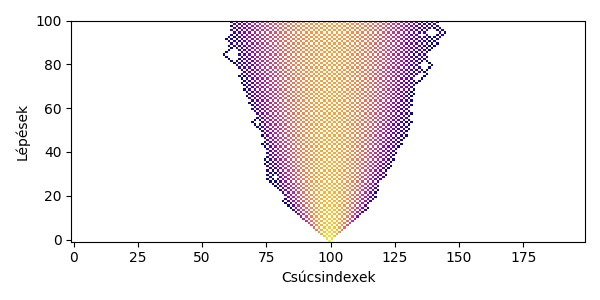
\includegraphics[width=\linewidth]{./figures/quantum/classical_simulation_short.jpg}
    \caption{Klasszikus}
  \end{subfigure}
  \begin{subfigure}{.45\linewidth}
    \centering
    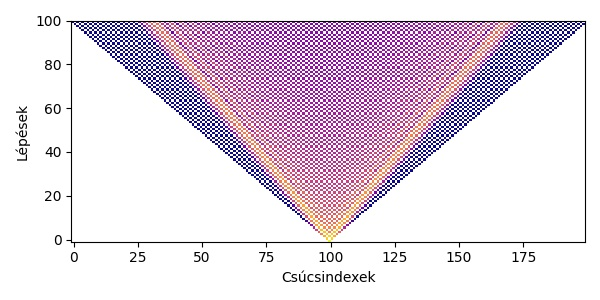
\includegraphics[width=\linewidth]{./figures/quantum/quantum_simulation_short.jpg}
    \caption{Kvantum}
  \end{subfigure}
\end{figure}

A fenti két ábra sokkal fakóbbnak tűnik, mint az eddig bemutatott szimulációs
ábrák, ez azért van így, mert nincs hurokél az egyenesen, tehát párosadik
lépésben csak páros indexű csúcsban, páratlanadik lépésben pedig csak páratlan
indexű csúcsban lehet a bolyongó. Így sakktáblaszerűen helyezkednek el a színes
és a fehér cellák az ábrákon.

A fenti eredmények összecsengnek a kvantumbolyongásokkal foglalkozó cikkek
által bemutatott eredményekkel a kvantum és a klasszikus bolyongás eloszlásaira
vonatkozóan.

\begin{figure}[H]
  \centering
  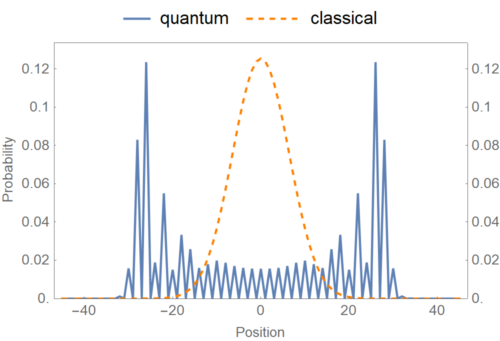
\includegraphics[width=0.5\linewidth]{./figures/quantum/teve.png}
  \caption{Eloszlások különbözősége \cite{VicPina}}
\end{figure}

\section{Bolyongás a szakaszon, klasszikus és kvantum esetben}

Ezek után azt is megvizsgáltam, hogy mi történik ha tovább futtatjuk a
szimulációkat, úgy hogy ha túllépnénk a megengedett koordinátákon, akkor
helyben maradunk. Másképpen fogalmazva, egy olyan szakaszon szimuláltam, aminek
a két végpontján hurokél van.

\begin{figure}[H]
  \centering
  \begin{subfigure}{.45\linewidth}
    \centering
    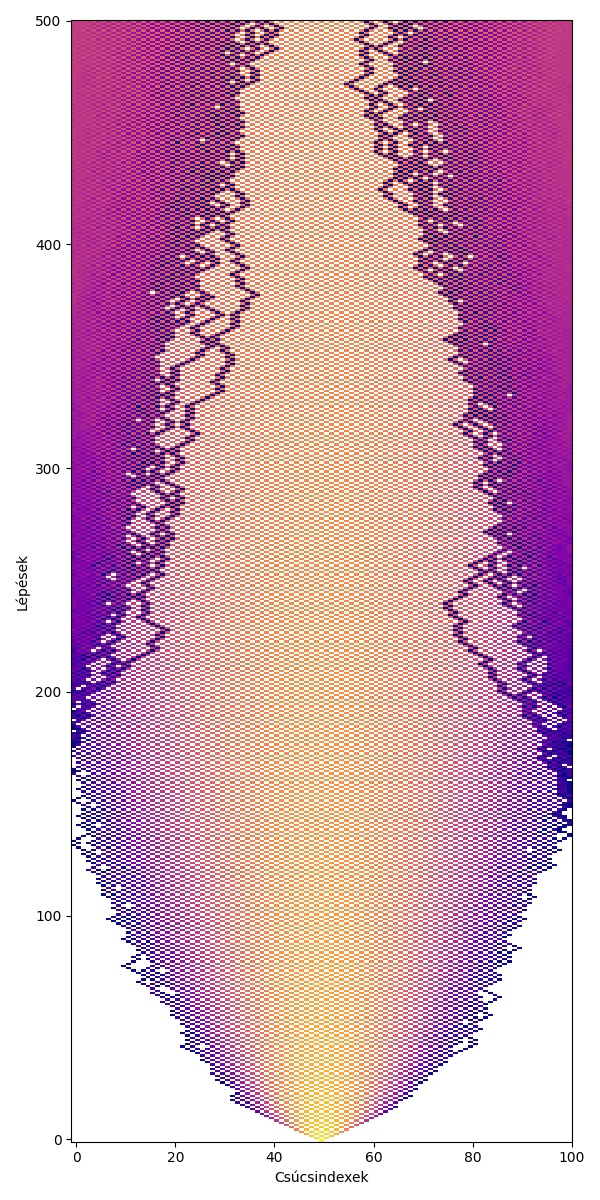
\includegraphics[width=\linewidth]{./figures/quantum/classical_simulation_long.jpg}
    \caption{Klasszikus}
  \end{subfigure}
  \begin{subfigure}{.45\linewidth}
    \centering
    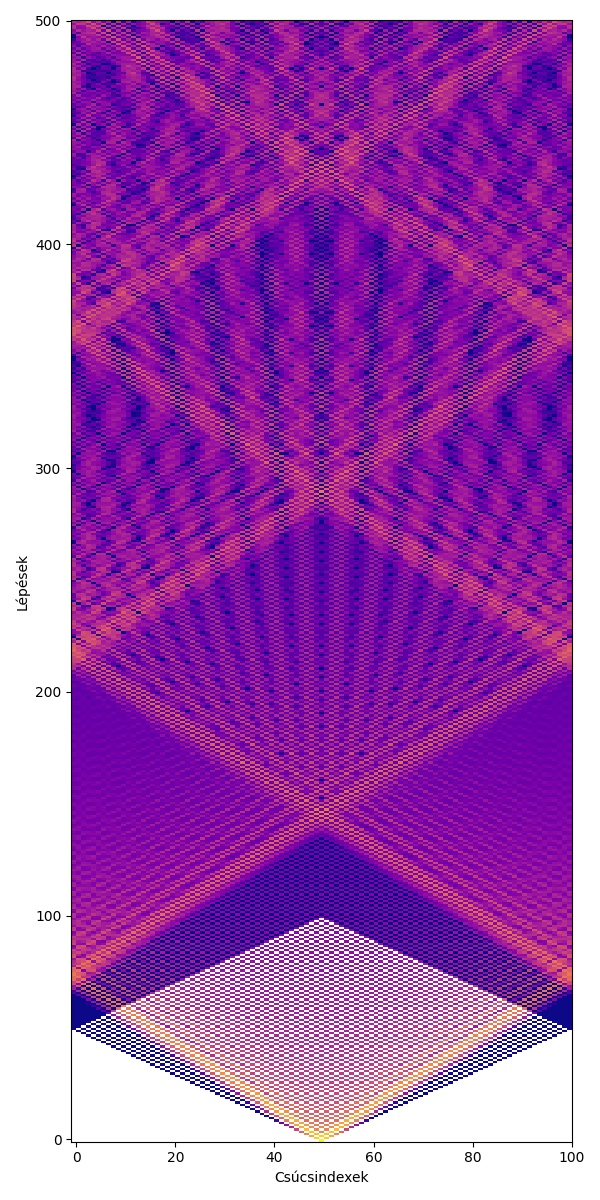
\includegraphics[width=\linewidth]{./figures/quantum/quantum_simulation_long.jpg}
    \caption{Kvantum}
  \end{subfigure}
\end{figure}

Nagyon érdekes csíkozott mintázat jött ki kvantum esetben. Ezen az ábrán az is
láthatóvá vált, hogy a két fő ,,púposodás'' mellett az eloszlásnak több kisebb
lokális maximuma is van, melyek egy rácsozott mintázatot eredményeznek.

\chapter{Zárszó, jövőbeli tervek}

Ebben a félévben elkészítettem egy olyan Pythonos keretrendszert, melyben
hatékonyan lehet gráfbolyongásos szimulációkat futtatni nevesített
részgráfokból álló gráfokon, továbbá megismertem és kipróbáltam a
kvantumbolyongás egy speciális esetét, 2-reguláris gráfra. A jövőben szeretném
bővíteni a programomat, először k-reguláris, majd általános gráfok
kvantumbolyongásának támogatásával, illetve a bolyongások matematikai
jellemzőinek (stacionárius eloszlás, keverési idő, elérési idők) számításával.
